%!TEX root = main.tex
Both \blk{rampgen} and \blk{buffer} require a current source, which in both cases done using a current mirror.
Those mirrors share the same bias voltage/current reference which is provided by \blk{vbias}
\sig{vbias} is chosen high ($\sim{2.5}{V}$) so that $|V_{ov}|$ is low in order to maximize the output range of the device.
It is generated using the circuit of figure~\ref{fig:vbias}.
\begin{figure}
  \centering
  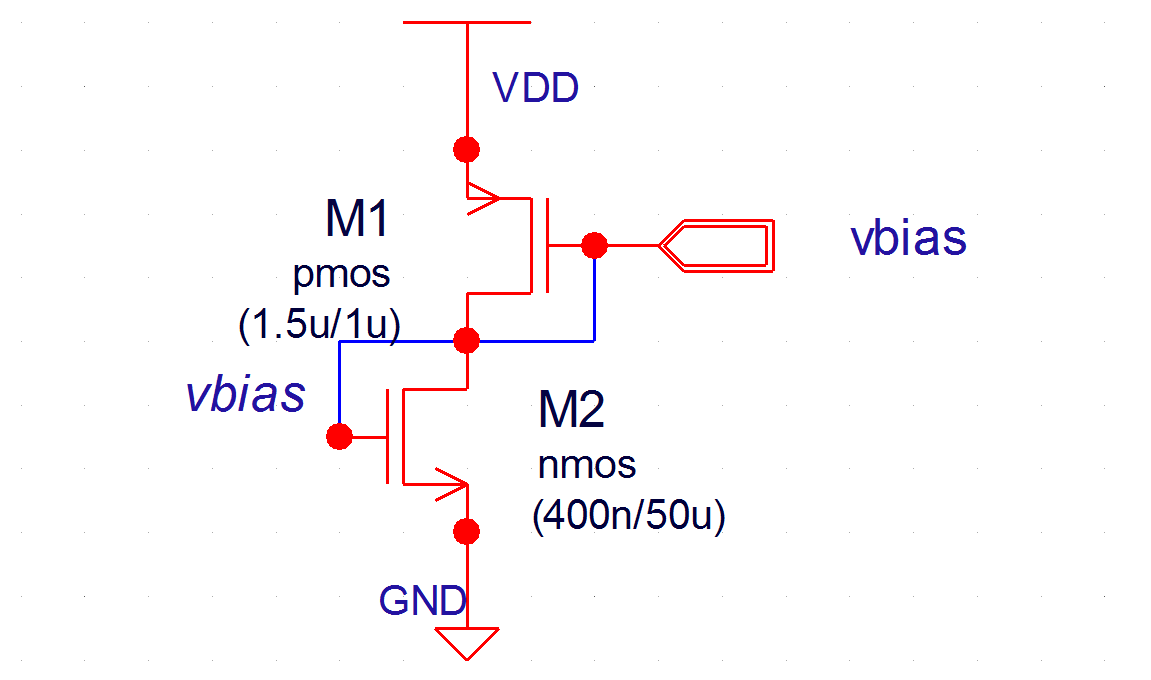
\includegraphics[width=\textwidth]{vbias.png}
  \caption{\blk{vbias} circuit.\label{fig:vbias}}
\end{figure}

\subsection{Sizing}
All the PMOS transistors in the mirrors share the same length \SI{2}{\micro\meter}. This is to minimize $g_{ds}$ and obtain good current source behaviour, and matching the lengths of the transistors in the mirrors reduces distortion and drift.

\sig{M2}'s width is chosen minimal in order to reduce the (useless) current consumed by \blk{vbias}. Moreover, increasing its width would mean increasing other dimensions in the circuit which is already contains large transistors in order keep the same output \sig{vbias}. \sig{M1}'s length being defined already, the prodcut $W_{\sig{M1}} \cdot L_{\sig{M2}}$ defines \sig{vbias}, which we try to obtain while keeping \sig{M2} at a reasonable length.
